\chapter{Strumenti}

\section{ROS}

ROS (Robot Operating System) è un framework flessibile usato per scrivere software per robot.
È una collezione di strumenti, librerie e convenzioni che ha lo scopo di semplificare la creazione di sistemi robot complessi e robusti in modo indipendente dalla piattaforma robotica. \\
ROS è costituito da una rete di processi che vengono eseguiti in parallelo e comunicano tra di loro in modo Peer-to-Peer.
Gli elementi principali che costituiscono il sistema sono:
\begin{itemize}
  \item \textbf{Nodi}: sono i processi che vengono eseguiti in parallelo.
  \item \textbf{Master}: è il server principale che si occupa di effettuare le operazioni di routing per permettere la comunicazione tra i diversi nodi.
  \item \textbf{Messaggi}: il contenuto che si scambiano i nodi. I messaggi possono essere sia di tipo standard sia definiti in modo custom.
  \item \textbf{Topic}: sono il canale di comunicazione usato dai nodi per permettere lo scambio di messaggi.
\end{itemize}
Il sistema di scambio dei messaggi si basa sull'architettura publisher/subscriber: ogni nodo può essere \textit{talker} (Publisher) o s \textit{listener}  (Subscriber).
I nodi talker creano il topic e pubblicano i messaggi su questo canale, mentre i nodi subscriber si sottoscrivono al topic e viene eseguita una callback ogni volta che viene ricevuto un messaggio. Più nodi subscriber si possono sottoscrivere allo stesso topic.

\begin{figure}[H]
\centering
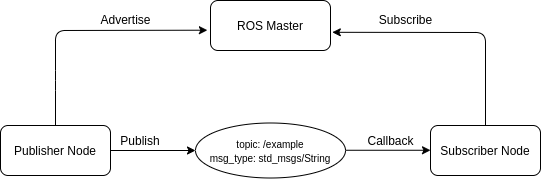
\includegraphics[scale=0.8]{images/ros_system.png}
\caption{Schema generale del sistema di comunicazione}
\end{figure}

Il software è open source ed è disponibile sul sito ufficiale \cite{ROS}, la versione usata per questo progetto è la Melodic.

\section{RVIZ}
RVIZ è un tool che permette la visualizzazione 3D dei messaggi scambiati da ROS. Usando questo strumento si può visualizzare in real-time la posizione del robot attraverso i dati dei sensori che vengono pubblicati.

\begin{figure}[H]
\centering
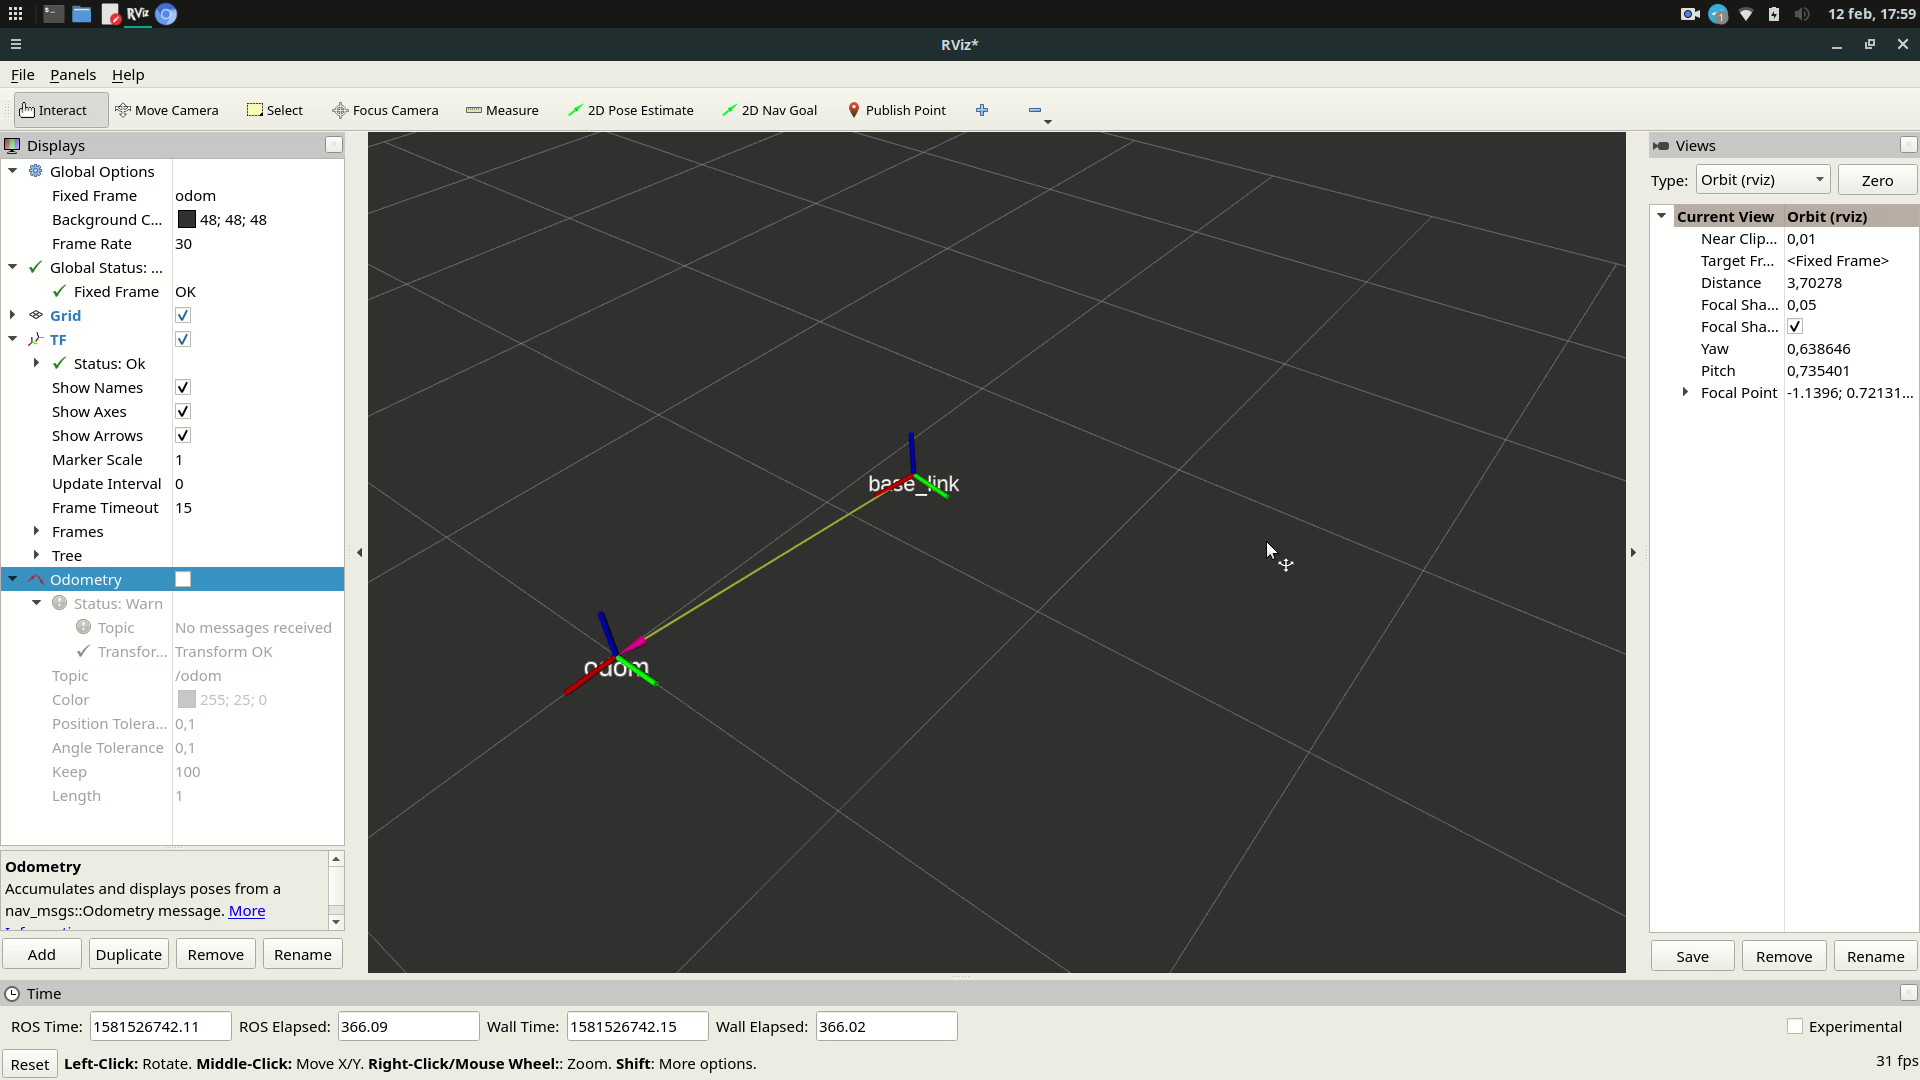
\includegraphics[scale=0.225]{images/rviz.png}
\caption{Visualizzazione di un robot nello spazio con RVIZ}
\end{figure}

\section{STM32CubeIDE}
STM32CubeIDE è un ambiente di sviluppo viluppato dalla ST Microelectronics per la programmazione e il debugging delle schede STM32. Il software è scaricabile gratuitamente dal sito ufficiale\cite{STM32CubeIDE}. \\
Le sue principali caratteristiche sono:
\begin{itemize}
    \item Toolchain GNU C/C++ per Arm e GDB debugger.
    \item Integrazione del tool STM32CubeMX per la generazione del codice di configurazione del sistema e delle periferiche del microcontrollore.
    \item Debugging avanzato che comprende feature come:
    \begin{itemize}
        \item Visualizzazione di CPU core, registri delle periferiche e memoria
        \item Visione delle variabili live 
        \item Analisi del sistema e tracing in tempo reale
        \item Tool di analisi dei CPU fault
    \end{itemize}
\end{itemize}

\begin{figure}[H]
\centering
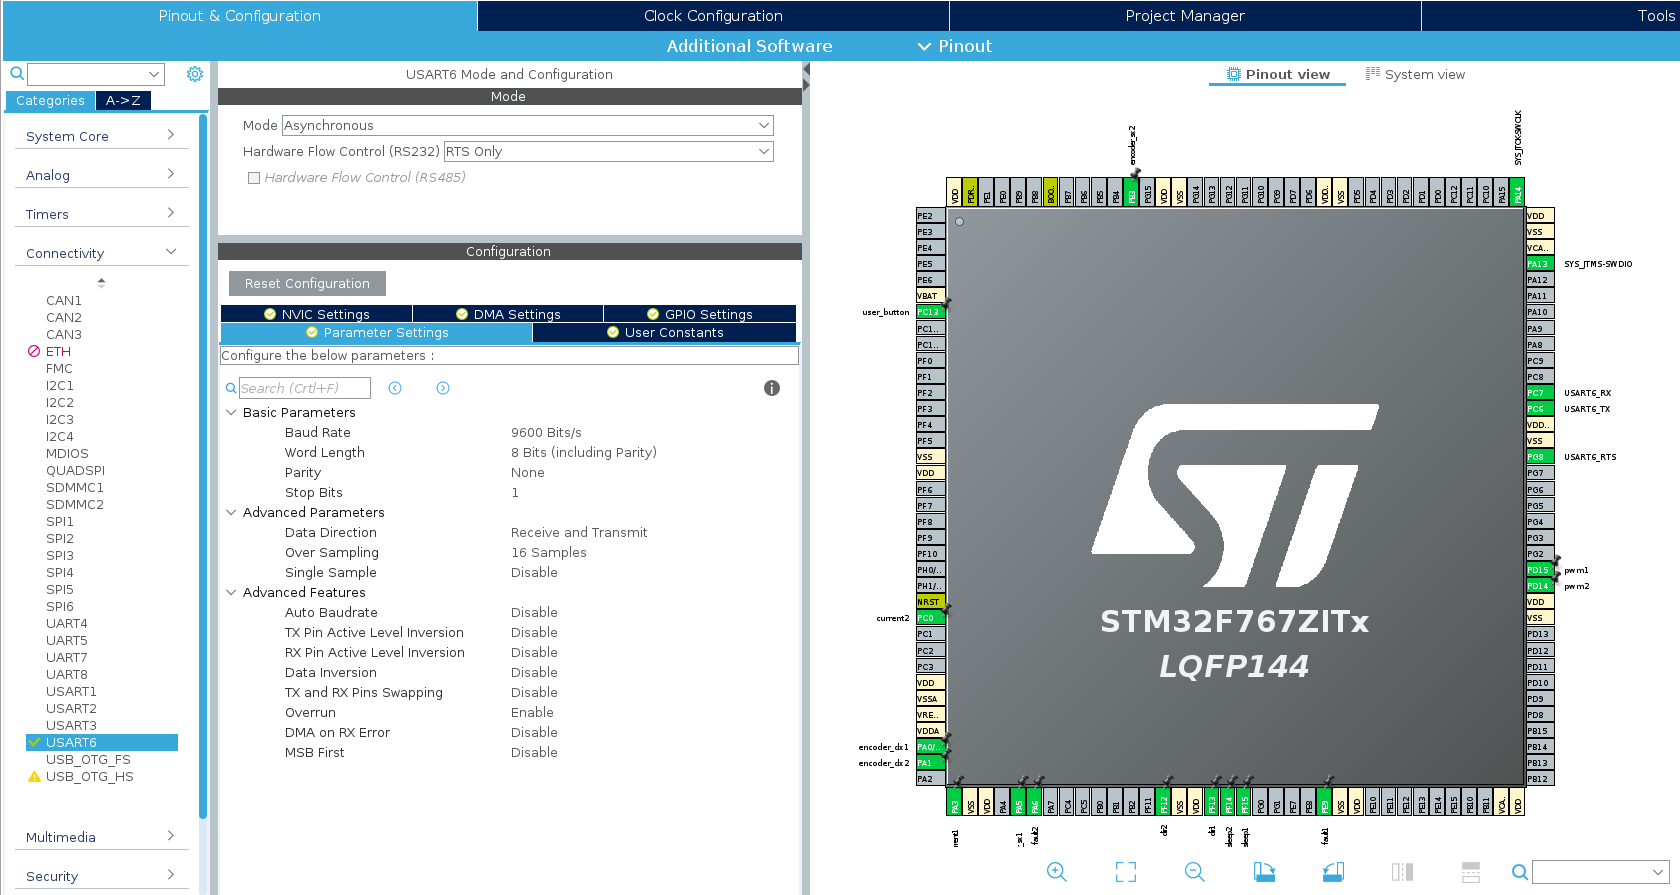
\includegraphics[scale=0.25]{images/stm32cubemx.png}
\caption{Cofigurazione di pinout e periferiche tramite lo strumento STM32CubeMX}
\end{figure}

\section{Protocol Buffers}
Protocol Buffers è un metodo di serializzazione dei dati strutturati, utile per lo sviluppo di software che necessita uno scambio di informazioni tra sistemi indipendenti.
La struttura dei dati viene descritta in un file di tipo \textit{.proto}, dopo di che, attraverso la compilazione con il comando \textit{protoc} e specificando il linguaggio di programmazione desiderato, vengono generate le classi per accedere ai dati. \\

\lstinputlisting[language=protobuf2, 
                style=protobuf,
                caption={Esempio di definizione di un messaggio con Protocol Buffers},
                captionpos=b]{codice/esempio.proto}
                
Protocol Buffers è sviluppato da Google e rilasciato con licenza open source \cite{ProtocolBuffers}. \\
Per questo progetto è stata utilizzata anche un'implementazione in C pensata per i microcontrollori, \textit{nanopb} \cite{nanopb}.

\section{sigrok Pulseview}
sigrok è una suite di software per l'analisi dei segnali, sfruttando dispositivi come oscilloscopi e analizzatori logici. \\
Pulseview è l'interfaccia grafica usata per sfrutttare questi tool e permette di interfacciarsi con i dispositivi sopracitati visualizzando il segnale in tempo reale, analizzandone i tempi e consente inoltre la decodifica di segnali digitali.
In particolare per questo progetto è stato usato Pulseview con un analizzatore logico per facilitare il debugging nella trasmissione dei segnali, ad esempio la trasmissione seriale di messaggi.

\begin{figure}[H]
\centering
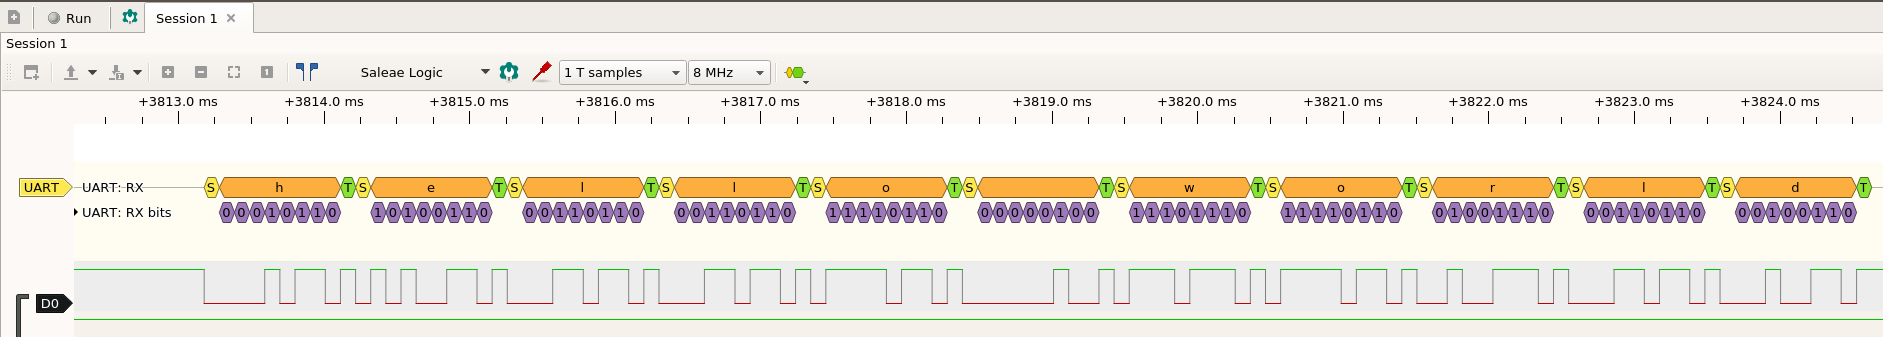
\includegraphics[scale=0.25]{images/pulseview.png}
\caption{Acquisizione e decodifica di un segnale UART}
\end{figure}

Pulseview è un progetto open source e liberamente scaricabile dal sito ufficiale\cite{Pulseview}.